\documentclass[
	% -- opções da classe memoir --
	12pt,				% tamanho da fonte
	% openright,			% capítulos começam em pág ímpar (insere página vazia caso preciso)
    oneside,			% para impressão somente frente. Oposto a twoside (frente e verso)
	a4paper,			% tamanho do papel. 
	% -- opções da classe abntex2 --
	%chapter=TITLE,		% títulos de capítulos convertidos em letras maiúsculas
	%section=TITLE,		% títulos de seções convertidos em letras maiúsculas
	%subsection=TITLE,	% títulos de subseções convertidos em letras maiúsculas
	%subsubsection=TITLE,% títulos de subsubseções convertidos em letras maiúsculas
	% -- opções do pacote babel --
	english,			% idioma adicional para hifenização
	%french,				% idioma adicional para hifenização
	%spanish,			% idioma adicional para hifenização
	brazil,				% o último idioma é o principal do documento
	]{abntex2}


% ---
% PACOTES
% ---

% ---
% Pacotes fundamentais 
% ---
\usepackage{cmap}				% Mapear caracteres especiais no PDF
\usepackage{lmodern}			% Usa a fonte Latin Modern
%\usepackage{helvet}			% Usa a fonte helvet(ARIAL)
%\usepackage{pslatex}			
\usepackage[T1]{fontenc}		% Selecao de codigos de fonte.
\usepackage[utf8]{inputenc}		% Codificacao do documento (conversão automática dos acentos)
\usepackage{indentfirst}		% Indenta o primeiro parágrafo de cada seção.
\usepackage{color}				% Controle das cores
\usepackage{graphicx}			% Inclusão de gráficos
\usepackage{enumerate}

% ---
% Pacotes adicionais, usados no anexo do modelo de folha de identificação
% ---
\usepackage{multicol}
\usepackage{multirow}
% ---

% Permite incluir listagens de código com o comando \lstinputlisting{}.
\usepackage{listings}
\usepackage{caption}
\DeclareCaptionFont{white}{\color{white}}
\DeclareCaptionFormat{listing}{\colorbox{gray}{\parbox{\textwidth}{#1#2#3}}}
\captionsetup[lstlisting]{format=listing,labelfont=white,textfont=white}
\renewcommand{\lstlistingname}{Listagem}
\definecolor{mygray}{rgb}{0.5,0.5,0.5}
\lstset{
	basicstyle=\scriptsize,
	breaklines=true,
%	numbers=left,
	numbersep=5pt,
	numberstyle=\tiny\color{mygray}, 
	rulecolor=\color{black},
	showstringspaces=false,
	tabsize=4,
    inputencoding=utf8,
    extendedchars=true,
    literate=%
    {é}{{\'{e}}}1
    {è}{{\`{e}}}1
    {ê}{{\^{e}}}1
    {ë}{{\¨{e}}}1
    {É}{{\'{E}}}1
    {Ê}{{\^{E}}}1
    {û}{{\^{u}}}1
    {ù}{{\`{u}}}1
    {â}{{\^{a}}}1
    {à}{{\`{a}}}1
    {á}{{\'{a}}}1
    {ã}{{\~{a}}}1
    {Á}{{\'{A}}}1
    {Â}{{\^{A}}}1
    {Ã}{{\~{A}}}1
    {ç}{{\c{c}}}1
    {Ç}{{\c{C}}}1
    {õ}{{\~{o}}}1
    {ó}{{\'{o}}}1
    {ô}{{\^{o}}}1
    {Õ}{{\~{O}}}1
    {Ó}{{\'{O}}}1
    {Ô}{{\^{O}}}1
    {î}{{\^{i}}}1
    {Î}{{\^{I}}}1
    {í}{{\'{i}}}1
    {Í}{{\~{Í}}}1
}

	
% ---
% Pacotes adicionais, usados apenas no âmbito do Modelo Canônico do abnteX2
% ---
\usepackage{lipsum}				% para geração de dummy text
% ---

% ---
% Pacotes de citações
% ---
\usepackage[brazilian,hyperpageref]{backref}	 % Paginas com as citações na bibl
\usepackage[alf]{abntex2cite}	% Citações padrão ABNT

% --- 
% CONFIGURAÇÕES DE PACOTES
% --- 

% ---
% Configurações do pacote backref
% Usado sem a opção hyperpageref de backref
\renewcommand{\backrefpagesname}{Citado na(s) página(s):~}
% Texto padrão antes do número das páginas
\renewcommand{\backref}{}
% Define os textos da citação
\renewcommand*{\backrefalt}[4]{
	\ifcase #1 %
		Nenhuma citação no texto.%
	\or
		Citado na página #2.%
	\else
		Citado #1 vezes nas páginas #2.%
	\fi}%
% ---

% ---
% Informações de dados para CAPA e FOLHA DE ROSTO
% ---
\titulo{Relatório do 2º Trabalho de Processamento Paralelo e Distribuído}
\autor{Leonardo Santos Paulucio}
\local{Vitória - ES}
\data{05 de Julho de 2018}
\instituicao{%
  Universidade Federal do Espírito Santo
  %\par
  %Setor Palotina
  \par
  Engenharia da Computação}
\tipotrabalho{Relatório técnico}
% O preambulo deve conter o tipo do trabalho, o objetivo, 
% o nome da instituição e a área de concentração 
\preambulo{Trabalho apresentado à disciplina de Processamento Paralelo e Distribuído do curso Engenharia da Computação da Universidade Federal do Espírito Santo como requisito parcial de avaliação.
\newline \newline \textbf{Professor:} João Paulo A. Almeida}

% ---

% ---
% Configurações de aparência do PDF final

% alterando o aspecto da cor azul
%\definecolor{blue}{RGB}{41,5,195}
\definecolor{blue}{RGB}{0,0,0}

% informações do PDF
\makeatletter
\hypersetup{
     	%pagebackref=true,
		pdftitle={\@title}, 
		pdfauthor={\@author},
    	pdfsubject={\imprimirpreambulo},
	    pdfcreator={LaTeX with abnTeX2},
		pdfkeywords={abnt}{latex}{abntex}{abntex2}{relatório técnico}, 
		colorlinks=true,       		% false: boxed links; true: colored links
    	linkcolor=blue,          	% color of internal links
    	citecolor=blue,        		% color of links to bibliography
    	filecolor=magenta,      		% color of file links
		urlcolor=blue,
		bookmarksdepth=4
}
\makeatother
% --- 

% --- 
% Espaçamentos entre linhas e parágrafos 
% --- 

% O tamanho do parágrafo é dado por:
\setlength{\parindent}{1.3cm}

% Controle do espaçamento entre um parágrafo e outro:
\setlength{\parskip}{0.2cm}  % tente também \onelineskip

% ---
% compila o indice
% ---
\makeindex
% ---

% ----
% Início do documento
% ----
\begin{document}

% Retira espaço extra obsoleto entre as frases.
\frenchspacing 

% ----------------------------------------------------------
% ELEMENTOS PRÉ-TEXTUAIS
% ----------------------------------------------------------
% \pretextual

% ---
% Capa
% ---
\imprimircapa
% ---

% ---
% Folha de rosto
% (o * indica que haverá a ficha bibliográfica)
% ---
\imprimirfolhaderosto*
% ---

% ---
% RESUMO
% ---

% resumo na língua vernácula (obrigatório)
% \begin{resumo} %% AQUI COMEÇA A PÁGINA DE RESUMO
% Costuma-se dizer que, numa economia capitalista, os problemas econômicos relativos à decisão sobre que tipos de produtos devem ser produzidos e a que preços serão vendidos esses produtos são resolvidos normalmente pelo livre jogo das forças de mercado – isto é, pelo livre funcionamento da oferta e da demanda. Nesta hipótese, as decisões e escolhas econômicas são individualizadas e feitas pelos consumidores – que são os demandantes dos bens e serviços – e pelos produtores – que são os ofertantes. Agindo de acordo com seus próprios interesses, os indivíduos, afetando e sendo afetados pelo sistema de preços, tomam as decisões que maximizarão a satisfação coletiva. 
% O objetivo é o de explicar de maneira simplificada como atua um sistema de preços e sua influência na alocação de recursos escassos.
% Ocorre, porém, que a determinação do preço e da quantidade produzida de um bem ou serviço depende essencialmente do número de agentes econômicos – demandantes e ofertantes – existentes nesse mercado. Por isso, é interessante caracterizar, antes, os diversos tipos de mercado existentes.
% O mercado, como você sabe, é o local onde se encontram os vendedores e compradores de determinados bens e serviços. Antigamente, a palavra mercado tinha uma conotação estritamente geográfica, mas isso já está deixando de ser assim. Hoje, com os avanços tecnológicos nas comunicações, as transações econômicas podem se realizar sem contato pessoal direto entre comprador e vendedor, tal como ocorre nas compras e vendas pela internet.


%  \vspace{\onelineskip}
    
%  \noindent
%  \textbf{Palavras-chaves}: latex. abntex. editoração de texto.
% \end{resumo} %AQUI TERMINA A PÁGINA DE RESUMO
% ---

% ---
% inserir lista de ilustrações
% ---

%\listoffigures* %% o * indica que não será incluso no sumário
%\cleardoublepage %% Pula página
% ---

% ---
% inserir lista de tabelas
% ---

%\listoftables*
%\cleardoublepage
% ---

% ---
% inserir lista de abreviaturas e siglas
% ---
%\begin{siglas}
%  \item[Fig.] Area of the $i^{th}$ component
%  \item[456] Isto é um número
%  \item[123] Isto é outro número
%  \item[lauro cesar] este é o meu nome
%\end{siglas}
% ---

% ---
% inserir lista de símbolos
% ---
%\begin{simbolos}
%  \item[$ \Gamma $] Letra grega Gama
%  \item[$ \Lambda $] Lambda
%  \item[$ \zeta $] Letra grega minúscula zeta
%  \item[$ \in $] Pertence
%\end{simbolos}
% ---

% ---
% inserir o sumario
% ---

\tableofcontents*

% ---

% ----------------------------------------------------------
% ELEMENTOS TEXTUAIS  (necessário para incluir número nas páginas)
% ----------------------------------------------------------
\textual

% ----------------------------------------------------------
% Introdução
% ----------------------------------------------------------
\chapter{Introdução} 

Com o crescente desenvolvimento dos sistemas distribuídos nos últimos tempos surgiu a necessidade de serviços que independem de um acoplamento direto entre remetente e destinatário. Para que essa comunicação aconteça, se faz necessário o uso de um intermediário. Através dele é possível se obter duas características importantes: desacoplamento espacial e desacoplamento temporal.

O desacoplamento espacial permite que as entidades remetentes e destinatárias não precisam se conhecer. Isso permite que os desenvolvedores possam usar a tecnologia de desenvolvimento que acharem melhor. Como hoje existe uma gama enorme de ferramentas, essa propriedade fornece ao desenvolvedor um grau de liberdade imenso.

Já o desacoplamento temporal permite que as entidades possam ter tempos de vida independentes umas das outras, isso garante que elas não precisam estar ativas ao mesmo tempo para poderem realizar a troca de mensagens.

Todas essas características tornam a comunicação indireta uma ferramenta muito usada em ambientes móveis/WEB e ambientes voltados a ocorrência de eventos. Como exemplo, pode se citar os \textit{Web Services}.

Os \textit{Web Services} permitem uma integração de sistemas e na troca de informações entre diferentes aplicações, permitindo que sistemas criados em plataformas totalmente diferentes sejam compatíveis. Para isso, a aplicação usa uma linguagem universal para se comunicar através de um intermediário, atualmente pode se citar o XML, JSON, CSV e etc.

Esse trabalho tem por objetivo praticar programação paralela e distribuída usando a API Java JMS, além de 
realizar análises de desempenho em um cluster de computadores. 
Ele consistirá na implementação de uma arquitetura mestre/escravo para realizar um ataque de dicionário em uma mensagem criptografada utilizando troca de mensagens em duas filas.


\chapter{Implementação} 
A implementação do trabalho foi feita utilizando a IDE NetBeans 8.2. Foram criados vários pacotes para facilitar a organização 
do código e das implementações de cada elemento. O trabalho é composto dos seguintes pacotes:

\begin{itemize}

	\item \textbf{br.inf.ufes.ppd:} Nesse pacote estão as interfaces padrões com os serviços oferecidos pelo mestre,
	a classe \textit{Guess} e a classe \textit{SubAttackJob}.
	
	\item \textbf{br.inf.ufes.ppd.application:} Nesse pacote estão as aplicações propriamente ditas. Estão nesse pacote as
	aplicações de Cliente, Escravo e Mestre.

	\item \textbf{br.inf.ufes.ppd.implementation:} Nesse pacote se encontram as implementações das interfaces e das 
	funcionalidades do mestre e escravo. 
	
	\item \textbf{br.inf.ufes.ppd.utils:} Por fim, nesse pacote estão as funcionalidades de criptografia e descriptografia e 
	a de geração de dados em ".csv" para geração dos gráficos.
		

\end{itemize}

Para o correto funcionamento da aplicação mestre, desenvolvida nesse trabalho, sempre é necessário adicionar a seguinte diretiva ao comando de inicialização do mesmo.

\begin{center}
	\begin{lstlisting}
		-Djava.rmi.server.hostname=(IP DA MAQUINA HOST)
	\end{lstlisting}
\end{center}

Essa diretiva é necessária para que o Java RMI possa criar a referência correta ao exportar um objeto remoto. 

Outro comando que deve ser executado antes da inicialização de qualquer elemento é o \textit{rmiregistry}. Ele deve ser
executado dentro da pasta raiz onde se encontram as classes, no caso do NetBeans essa pasta é "build/classes/".
Nessa pasta se encontra a pasta raiz do pacote do trabalho, nesse caso a pasta "br".

\section{Cliente}

A aplicação cliente é a mesma implementada no 1º trabalho da disciplina e não foi alterada nenhuma parte do código. O programa cliente recebe como argumentos: o nome do arquivo criptografado, o trecho conhecido do texto original, um terceiro parâmetro que indica o tamanho do vetor de \textit{bytes} aleatório que será gerado em caso do arquivo criptografado não existir, e por último o dicionário de chaves.

Assim, o cliente é responsável por localizar o mestre utilizando o \textit{Registry}(utilizando a funcionalidade de \textit{lookup}) e solicitar o serviço de ataque através do método \textit{attack}. Ao solicitar o serviço, o cliente passa o arquivo criptografado e o trecho conhecido, ficando bloqueado enquanto aguarda uma resposta do mestre.

Caso o nome do arquivo, fornecido como argumento para o programa cliente, seja inválido ele fica responsável por gerar um vetor aleatório de bytes, cujo tamanho será igual ao 3º parâmetro fornecido ou, caso esse não exista, será usado um tamanho aleatório na faixa de 1Kb a 100Kb.

O comando utilizado para iniciar o cliente é:

\begin{lstlisting}
	java br.inf.ufes.ppd.application.Client <Arquivo> <Trecho> <Tam.Vetor> <Dicionario>
\end{lstlisting}


\section{Escravo}
O escravo recebe como parâmetros: o caminho para o arquivo de dicionário, o nome do escravo que será criado e endereço do \textit{host} onde está hospedado o \textit{Glassfish}. Caso alguns desses parâmetros não sejam fornecidos ele pega seus valores padrões existentes em um arquivo de configurações.

Inicialmente, o escravo se conecta ao \textit{Glassfish} que está rodando no \textit{host} especificado para obter uma \textit{Connection Factory}, e assim, as filas onde serão colocadas os subataques e os \textit{guesses}. Após terminar essas tarefas de inicialização, o escravo fica ocioso esperando algum subataque ser adicionado na fila, para que, assim, possa iniciar o processamento. 

Cada escravo realiza apenas um trabalho por vez, ou seja, quando existe um trabalho na fila o escravo o retira para realizar o processamento, e, somente quando esse trabalho é finalizado ele verifica na fila novamente se existe um novo trabalho para poder executar. Durante o processamento caso algum \textit{Guess} seja encontrado o escravo o adiciona à fila de \textit{Guesses} para que o mestre possa processar e montar a resposta que será enviada ao cliente.

O comando para se iniciar um escravo é:

\begin{lstlisting}
	java br.inf.ufes.ppd.application.SlaveServer <Dicionario> <Escravo> <Host>
\end{lstlisting}

É importante falar que para que a aplicação \textit{SlaveServer} possa ser executada é necessário adicionar o arquivo \textit{<gf-client.jar>} ao \textit{classpath}. Caso esse arquivo já não esteja no diretório local deve se usar a seguinte diretiva na linha de comando(antes do nome da aplicação mostrado acima), para adicioná-lo:

\begin{lstlisting}
	java -cp .:../../glassfish5/glassfish/lib/gf-client.jar br.inf ...
\end{lstlisting}


\section{Mestre}

O mestre recebe como parâmetro o endereço do \textit{registry} e do \textit{host} onde está o \textit{Glassfish}, caso eles não sejam fornecidos são utilizados os valores padrões existentes no arquivo de configurações.

O mestre é a aplicação que fornece o serviço de \textit{attack} para um cliente. Quando esse serviço é solicitado
ele cria vários subataques - o número de subataques depende de uma variável \textit{M} que determina o tamanho do intervalo dos índices de cada trabalho - adicionando-os na respectiva fila, para que, os escravos possam pegar a tarefa e executar.
O mestre fica sempre monitorando a fila de \textit{Guesses}, através de uma \textit{thread}, para processar os resultados obtidos pelos escravos de forma que seja possível montar a resposta ao final do ataque para o cliente.
Quando todos os subataques são finalizados pelos escravos o mestre envia a resposta para o cliente com todos os resultados encontrados durante os subataques.

O comando para se iniciar um escravo é:

\begin{lstlisting}
	java br.inf.ufes.ppd.application.MasterServer <registry> <host>
\end{lstlisting}

Da mesma forma que foi explicado anteriormente para o escravo, é necessário adicionar o arquivo \textit{<gf-client.jar>} ao \textit{classpath} utilizando o comando:

\begin{lstlisting}
	java -cp .:../../glassfish5/glassfish/lib/gf-client.jar br.inf ...
\end{lstlisting}

Nas próxima seções serão discutidos os principais pontos da estrutura de dados utilizada no trabalho, decisões de projeto e 
problemas que ocorreram durante a implementação.

\section{Estrutura de Dados}

Como o cliente não precisou ser alterado, sua estrutura é a mesma do 1º trabalho. Ela é bem simples e não possui nada muito complexo já que sua função é, basicamente, localizar um mestre para solicitar o serviço de ataque enviando o arquivo criptografado e o trecho conhecido, após isso, fica bloqueado aguardando uma resposta do mestre. Sendo assim, sua estrutura não será discutida em detalhes.

O escravo sofreu alterações com a implementação feita no trabalho anterior. Sua estrutura ficou mais simples, visto que a operação de \textit{checkpoint} e \textit{rebind} não são mais necessárias. A única informação que o escravo possui é seu nome  e uma lista de chaves candidatas, que são lidas de um arquivo de dicionário. Ao pegar um trabalho da fila ele percorre o intervalo de índices indicados na mensagem verificando se alguma dela produz uma mensagem com o trecho conhecido. Caso exista, ele produz um \textit{Guess} e o adiciona a fila de \textit{Guesses} para que o mestre possa pegar.

Com as alterações exigidas para o mestre, sua implementação também ficou mais simples, já que não se fez necessário realizar o gerenciamento de escravos e recuperação de erros. Basicamente o mestre recebe uma requisição de ataque de um cliente e cria vários \textit{jobs} para esse ataque colocando-os na fila de subataques para que os escravos possam pegar. Quando uma requisição é recebida pelo mestre ele cria uma \textit{thread} para gerar os \textit{jobs}, isso permite que ele possa receber requisições em paralelo.

Para a implementação do mestre foi criada uma estrutura de controle de ataque chamada \textit{AttackControl}.
Essa estrutura é responsável por possuir as informações de um ataque solicitado por um cliente. Ele possui: a informação do tempo em que o ataque começou, possui uma variável que diz se o ataque está terminado, uma referência para a mensagem criptografada e para o trecho conhecido daquele ataque e por fim uma 	\textit{HashMap} com os respectivos subataques e o \textit{status} de cada um, indicando se o subataque já terminou ou não.
	
Para acessar as estruturas o mestre possui \textit{HashMaps}, que facilitam o acesso e localização das mesmas. 
Essas \textit{HashMaps} são as seguintes:

\begin{itemize}

	\item \textbf{HashMap de AtaqueID em Lista de \textit{Guess}:} Esse mapeamento permite que dado um número de ataque o
	mestre obtenha a lista de \textit{guess} desse ataque.
	
	\item \textbf{HashMap de SubataqueID em AtaqueID:} Esse mapeamento permite ao mestre saber qual é o ataque que um 
	subataque faz parte.
	
	\item \textbf{HashMap de AtaqueID em AttackControl:} Esse mapeamento permite que o mestre obtenha o
	\textit{AttackControl} de um número de ataque.
	
\end{itemize}

Uma outra ferramenta utilizada na implementação do mestre é o \textit{synchronized} de Java, que faz com que o acesso
a uma determinada variável seja serializado. Essa ferramenta é de extrema importância para o mestre, visto que ele pode
receber várias solicitações de ataque em paralelo, e o acesso a algumas estruturas se não forem serializados podem gerar
exceção de acesso concorrente.

Para a troca de mensagens entre o mestre-escravo e escravo-mestre foi utilizado o \textit{ObjectMessage}, que permite enviar um objeto em forma de mensagem, desde que esse objeto implemente o \textit{Serializable} de Java, sendo assim, foram criadas duas classes para isso, são elas:

\begin{itemize}

	\item \textbf{SubAttackJob:} Essa estrutura é utilizado na troca de mensagens do mestre para os escravos através da fila.
	É responsável por possuir as informações de um subataque criado pelo mestre, assim, possui: uma referência para a
	mensagem criptografada e para o trecho conhecido daquele ataque, o índice inicial e final que deve ser percorrido para
	aquele subataque, e por fim, o número do subataque.
		
	\item \textbf{Guess:} Essa estrutura é responsável pela troca de mensagens do escravo para o mestre.
	Ela possui a chave candidata, a mensagem decriptografada, o nome do escravo que encontrou a chave, o número do ataque e 
	uma variável \textit{booleana} que indica se aquele ataque acabou.
		
\end{itemize}

\section{Decisões de Projeto}
Durante a implementação do projeto algumas decisões tiveram que ser tomadas, elas estão discutidas a seguir.

\begin{enumerate}

	\item \textbf{Lista separada de \textit{guess}}: A decisão de usar uma lista separada para os \textit{guesses} foi 
	basicamente por já ter sido usada e dado certo no 1º trabalho. Com essa estrutura fica simples o gerenciamento dos 
	\textit{guesses} obtidos, de forma que fica fácil montar a mensagem que será enviada ao cliente ao término do ataque.
	
	\item \textbf{Criação de subataques:} Da mesma forma que para o item anterior, a criação de subataques foi usada no 1º 	
	trabalho, e se encaixou perfeitamente nesse segundo trabalho, permitindo uma grande facilidade no gerenciamento dos 
	subataques criados para um dado ataque. Isso facilitou na forma de verificar se um ataque já tinha terminado, pois 
	bastava verificar se todos os subataques de um ataque já tinham terminado.
		
	\item \textbf{Fim de um Subataque:}  Para determinar o final de um subataque foi usada a mesma classe \textit{Guess}
	com os atributos vazios, com exceção do número do ataque e a variável \textit{booleana} que representa o fim do ataque 		que era setada para \textit{true}, dessa forma, quando o mestre pegava uma mensagem da fila a primeira coisa que ele faz 
	ao desempacotar a mensagem é verificar a variável \textit{booleana}, caso seja \textit{false} é um \textit{Guess}, 
	caso contrário é uma mensagem indicando que o subataque acabou.
	
\end{enumerate}

\section{Problemas Durante a Implementação}
Durante a implementação desse trabalho não foram encontrados muitos problemas. Foi possível aproveitar algumas estruturas que foram usadas no 1º trabalho e também os problemas que surgiram já eram conhecidos pois ocorreram durante a implementação do trabalho anterior.

Um novo problema que ocorreu relacionado ao JMS foi que quando não se tinha nenhum escravo rodando e o mestre recebia uma requisição de um cliente e gerava os respectivos subataques esses ataques ficavam na fila, assim, ao se iniciar uma aplicação de escravo ele conseguia pegar o trabalho da fila, porém ao se iniciar outro escravo o segundo não pegava mais nenhum trabalho. Isso ocorria pois existe uma funcionalidade de \textit{prefetch} do \textit{Glassfish} que adiciona as mensagens a uma "cache" para cada escravo, porém ao se ajustar a configuração \textit{imqConsumerFlowLimitPrefetch} esse problema foi resolvido.

Outro problema que surgiu foi para limpar as filas durante os testes de implementação, pois ao se fechar as aplicações as mensagens continuavam na fila, e ao reiniciar a aplicação do mestre ocorria um erro pois aquele ataque não existia. Para resolver isso foi feito um ajuste no código para limpar a fila antes de iniciar.


\chapter{Análise de Desempenho} 

\section{Máquinas e Equipamentos Utilizados}

Para a análise de desempenho foram utilizados os computadores do laboratório de graduação (LabGrad I), que possuem as seguintes configurações: processador \textit{AMD Athlon(tm) Dual Core Processor 5000B} com 4GB de memória RAM e o Sistema Operacional utilizado foi o \textit{Ubuntu 16.04.4 LTS}. A configuração de rede das máquinas era o padrão Ethernet 100Mbps.

\section{Cenário A}

O cenário A consiste em 3 máquinas distintas, cada qual executando 4 aplicações de escravo, totalizando 12 escravos. A aplicação do mestre e do cliente foram executadas em uma outra máquina. Durante as medições procurou-se deixar a máquina com apenas as aplicações rodando para evitar possíveis ruídos, mas é bom lembrar que existiam os processos em \textit{background} do SO. 

Para a medição dos dados foi criada uma aplicação cliente para gerar tamanhos aleatórios de vetor de 0 a 60Kb, sendo que os
tamanhos foram espaçados de 5 em 5Kb.


%%%%%%%%%%%%%%%%%%%%%%%%%%%%%%%%%%%%%

A Figura \ref{fig:cent:tempo_respostaXtamanho_msg} apresenta um gráfico com o tempo de resposta obtido com diferentes tamanhos de mensagem para diferentes números de escravos em uma mesma máquina. É bom observar que o caso onde existe apenas um escravo é a medição obtida com uma aplicação centralizada que realiza o ataque sozinha.

Ao observar o gráfico percebe-se claramente que à medida que aumenta-se o número de escravos, ou seja, faz-se o paralelismo da 
execução da tarefa(já que foi utilizado apenas um computador), o tempo de resposta diminui como imaginado, visto que ao
realizar o paralelismo em um computador com mais de um \textit{core} de processamento espera-se que a tarefa seja executada
em um tempo menor.

Outro ponto interessante de se notar é o fato de que apesar de se aumentar o número de escravos a partir do momento em que se adiciona mais de 4 escravos o tempo de resposta não sofre muitas mudanças sendo aproximadamente o mesmo até 8 escravos. Isso
pode ser explicado pelo fato de que como a máquina possui apenas 4 \textit{cores} de processamento, não faria muito sentido o desempenho aumentar muito ao se colocar mais escravos do que o número de \textit{cores}, podendo até piorar por causa do \textit{overhead} de escalonamento de processos e devido aos processos do SO que rodam em \textit{background}.


\begin{figure}[!htb]
\centering
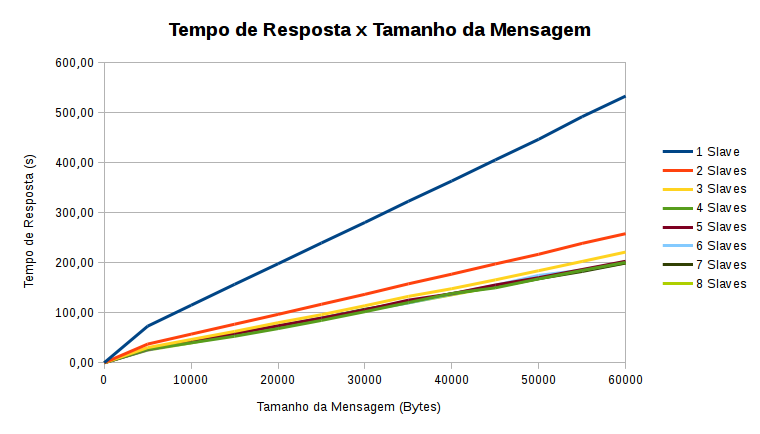
\includegraphics[scale=0.65]{figuras/temporesposta_centralizado.png}
\caption{Gráfico do Tempo de Resposta x Tamanho da Mensagem}
\label{fig:cent:tempo_respostaXtamanho_msg}
\end{figure}

A Figura \ref{fig:cent:speedupXtamanho_msg} apresenta o gráfico com o \textit{Speed Up} como função do tamanho da mensagem para diferentes números de escravos. Para se calcular o \textit{Speed Up} foi utilizado como tempo de execução serial o obtido pela aplicação centralizada.

Ao analisar o gráfico nota-se que à medida que o número de escravos aumenta o \textit{Speed Up} também vai aumentando, porém 
a partir de 4 escravos pra cima o seu valor varia muito pouco. Como visto em sala de aula verifica-se que o \textit{Speed Up}
obtido foi sublinear, o que era o esperado, pois segundo a Lei de Amdahl o maior \textit{Speed Up} que se consegue obter é o liner onde o \textit{Speed Up} é igual ao número de \textit{threads} de execução paralela, sendo que obter esse valor ótimo é
impossível visto que sempre existirá uma parte do programa que tem que ser executado serialmente, no caso desse trabalho o 
mestre é o que precisa executar algumas ações de forma serial.

\begin{figure}[!htb]
\centering
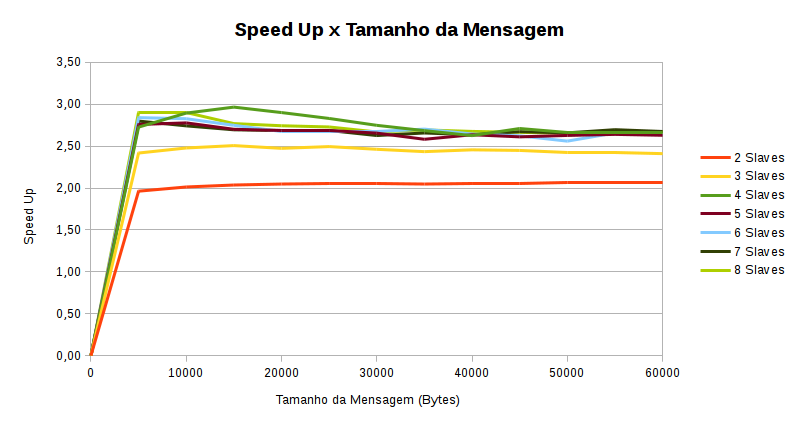
\includegraphics[scale=0.55]{figuras/speedup_centralizado.png}
\caption{Gráfico do Speed Up x Tamanho da Mensagem}
\label{fig:cent:speedupXtamanho_msg}
\end{figure}

A Figura \ref{fig:cent:eficienciaXtamanho_msg} apresenta o gráfico com a eficiência em função do tamanho da mensagem para 
diferentes números de escravos.

Ao observar o gráfico percebe-se claramente que quanto mais escravos são adicionados menor é a eficiência. Isso é esperado
visto que como observado na Figura \ref{fig:cent:speedupXtamanho_msg} à medida que aumenta-se o número de escravos o \textit{Speed Up} não se altera muito sendo o mesmo para mais do que 4 escravos com isso a eficiência tende a ser menor
para um número maior de escravos.

Um outro ponto a se destacar é que para 2 escravos e eficiência foi um pouco maior do que 1, isso é impossível pelo fato de
que a maior eficiência possível de se obter é 1. Isso pode ter ocorrido devido a ruídos que podem ter ocasionado em erros na
medição dos tempos.

\begin{figure}[!htb]
\centering
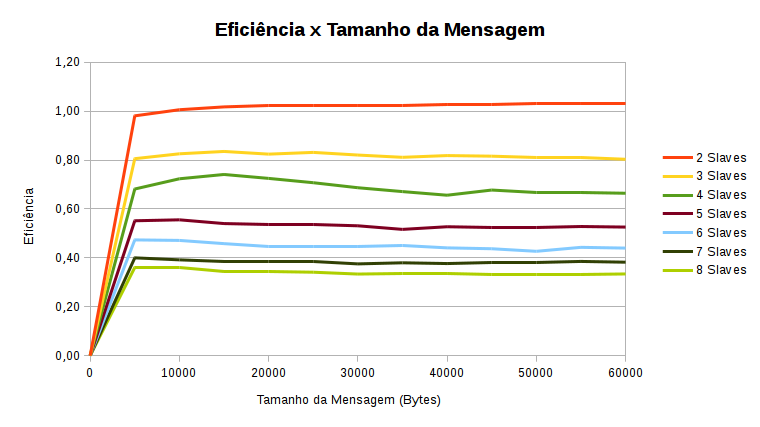
\includegraphics[scale=0.55]{figuras/eficiencia_centralizado.png}
\caption{Gráfico da Eficiência x Tamanho da Mensagem}
\label{fig:cent:eficienciaXtamanho_msg}
\end{figure}

Por fim, a Figura \ref{fig:cent:overheadXtamanho_msg} apresenta as medições do \textit{overhead} obtidos. Pode-se notar que 
o gráfico apresenta muita oscilação causada provavelmente por existirem processos do SO rodando em \textit{background}. Isso
faz com que não forneça informações tão relevantes, como os processos rodam na mesma máquina o \textit{overhead} é muito
pequeno sua medição acaba ficando refém dos ruídos.

\begin{figure}[!htb]
\centering
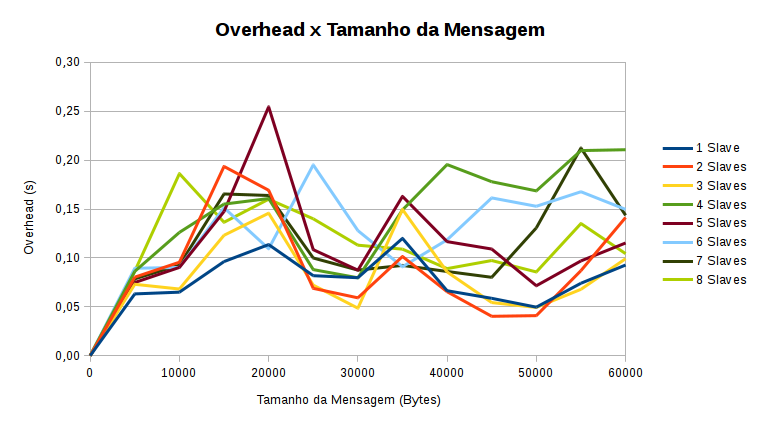
\includegraphics[scale=0.65]{figuras/overhead_centralizado.png}
\caption{Gráfico do Overhead x Tamanho da Mensagem}
\label{fig:cent:overheadXtamanho_msg}
\end{figure}


\section{Cenário B}

As medições para essa análise foram obtidas utilizando os computadores do LabGrad. Vale destacar que até os testes para a 
obtenção dos dados para 7 escravos o LabGrad estava com poucos alunos de graduação o que permitiu uma melhor medição dos tempos, porém ao se realizar a medição para 8 escravos, o LabGrad teve um problema de rede e quando foi resolvido haviam muitos alunos utilizando as máquinas, isso fez com que os dados obtidos para 8 escravos fossem prejudicados, porém mesmo com esse problema pode-se realizar uma análise do desempenho.

Para a medição dos dados também foi usada a aplicação cliente de teste para gerar tamanhos aleatórios de vetor de 0 a 60Kb,
sendo que os tamanhos foram espaçados de 5 em 5Kb.

Para os testes foram utilizados 4 máquinas. Para os testes até 4 escravos cada máquina possuía rodando apenas 1 escravo, para 5 escravos até 8 foram sendo adicionados escravos em cada uma dessas 4 máquinas de modo que ao final cada uma tivesse apenas 2
escravos rodando ao mesmo tempo. Essa estratégia foi usada pois cada computador possuía dois \textit{cores} de processamento.

A Figura \ref{fig:dist:tempo_respostaXtamanho_msg} apresenta um gráfico com o tempo de resposta obtido com diferentes tamanhos de mensagem para diferentes números de escravos de forma distribuída. Destaca-se que o caso onde existe apenas um escravo é a medição foi obtida com uma aplicação centralizada que realizou o ataque sozinha em uma das máquinas.

Ao observar o gráfico percebe-se claramente que à medida que aumenta-se o número de escravos, ou seja, faz-se a distribuição da tarefa entre as diferentes máquinas o tempo de resposta diminui como imaginado, como a tarefa será distribuída entre 
diferentes máquinas cada uma com uma pequena parte da tarefa espera-se que o processamento de cada parte seja mais rápido.
Destaca-se que o caso onde há apenas 1 escravo, foi medido rodando a mesma aplicação centralizada da análise anterior nas máquinas do LabGrad.

Uma observação interessante de se notar é que diferentemente do caso anterior onde se analisou o desempenho de paralelismo após a utilização de 4 escravos o tempo de resposta foi basicamente o mesmo para até 8 escravos. Já nesse caso distribuído 
nota-se que ao aumentar o número de escravos o tempo de resposta diminuiu para todos os escravos mesmo que a diferença entre 6 e 7 escravos seja pequena é possível observar uma diferença no tempo. Vale destacar novamente que para 8 escravos as medições foram prejudicadas pelo momento do teste e como não foi possível refazé-los eles apresentaram essa diferença. Mas acredita-se
que caso os problemas citados não tivessem ocorrido o grafíco apresentaria uma melhora mesmo que pequena no tempo de resposta
para o caso de 8 escravos.

\begin{figure}[!htb]
\centering
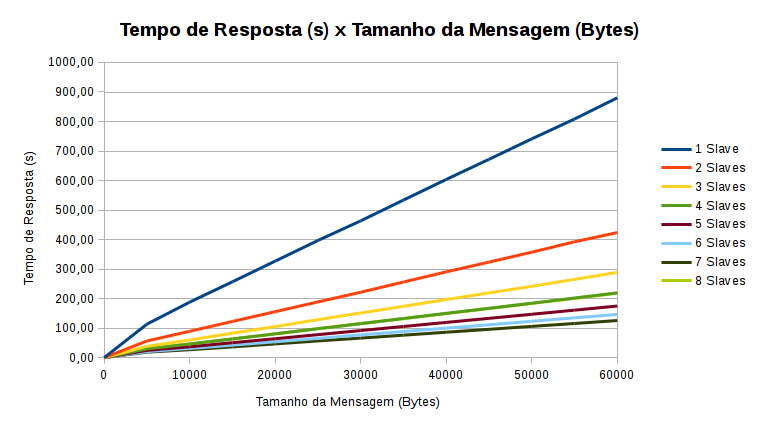
\includegraphics[scale=0.65]{figuras/temporesposta_distribuido.png}
\caption{Gráfico do Tempo de Resposta x Tamanho da Mensagem}
\label{fig:dist:tempo_respostaXtamanho_msg}
\end{figure}

A Figura \ref{fig:dist:speedupXtamanho_msg} apresenta o gráfico do \textit{Speed Up} em função do tamanho da mensagem para diferentes números de escravos. O tempo de execução serial utilizado para o cálculo foi o tempo de execução da aplicação centralizada nas máquinas do LabGrad.

Ao analisar o gráfico nota-se que à medida que o número de escravos aumenta o \textit{Speed Up} também vai aumentando, mas diferentemente da análise anterior eles não se aproximam de um valor em comum à medida que o número de escravos aumenta, sendo bem distintos. Para o caso de 8 escravos ele se equipara ao caso de 4 escravos devido aos problemas que ocorreram durante as medições. 

Como visto em sala de aula verifica-se que o \textit{Speed Up} obtido foi linear, o que inicialmente é estranho, já que 
esse é o máximo \textit{speed up} teórico possível.

Esse resultado pode ter sido obtido por alguns fatores:

\begin{itemize}
	\item Erros de medições dos tempos;
	\item O algoritmo sequencial não é o melhor que se pode conseguir;
	\item A lei de Amdahl considera que o caso serial é executado por um único processador, o que nesse caso não ocorre visto 
	que as máquinas possuem dois \textit{cores} de processamento, então mesmo que ela execute a tarefa sozinha o SO irá 
	dividi-lá entre os processadores.
\end{itemize}

\begin{figure}[!htb]
\centering
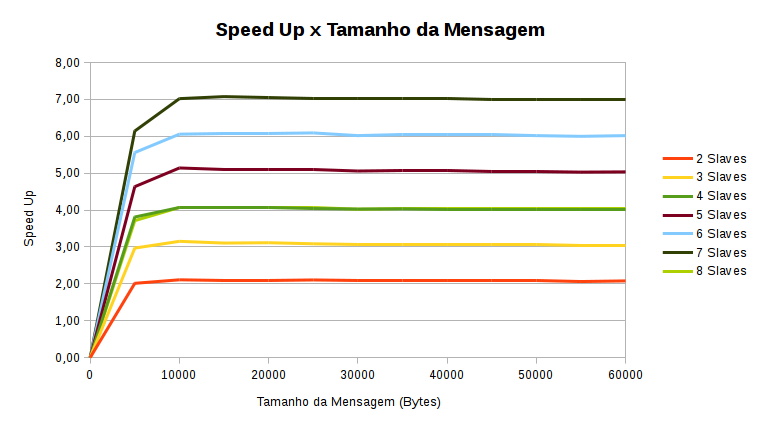
\includegraphics[scale=0.65]{figuras/speedup_distribuido.png}
\caption{Gráfico do Speed Up x Tamanho da Mensagem}
\label{fig:dist:speedupXtamanho_msg}
\end{figure}


A Figura \ref{fig:dist:eficienciaXtamanho_msg} apresenta a eficiência obtida para diferentes números de escravos. Percebe-se 
que a eficiência foi aproximadamente 1 para todos os casos, exceto para o de 8 escravos devido aos problemas já citados.

Percebe-se que a eficiência acaba oscilando para cima e para baixo de 1 isso pode ser ocasionado pelos mesmos problemas citados anteriormente para o \textit{Speed Up}. Com isso, considera-se aceitável os dados medidos já que eles não são muito
maiores do que o valor máximo possível que é 1.


\begin{figure}[!htb]
\centering
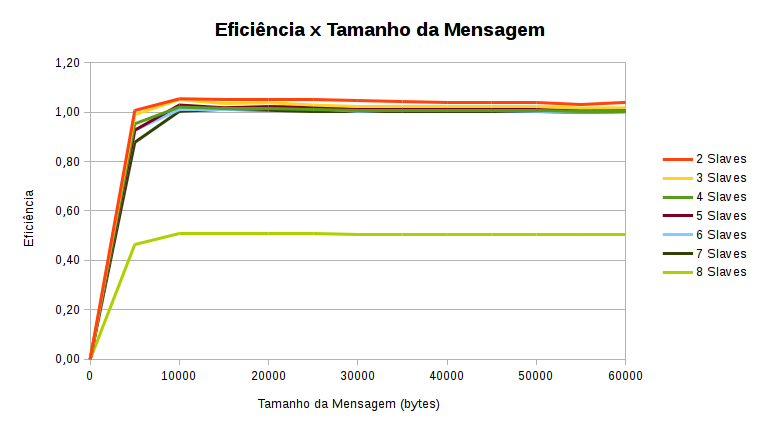
\includegraphics[scale=0.65]{figuras/eficiencia_distribuido.png}
\caption{Gráfico da Eficiência x Tamanho da Mensagem}
\label{fig:dist:eficienciaXtamanho_msg}
\end{figure}

A Figura \ref{fig:dist:overheadXtamanho_msg} apresenta o \textit{overhead} medido para diferentes números de escravos. 

Nesse caso observa-se uma oscilação ocasionada por ruídos da rede, mas mesmo com esse problema é possível verificar que à
medida que se aumenta o número de escravos o \textit{overhead} aumenta. O que é algo esperado visto que torna-se necessário 
enviar \textit{bytes} de dados para diferentes máquinas na rede.

\begin{figure}[!htb]
\centering
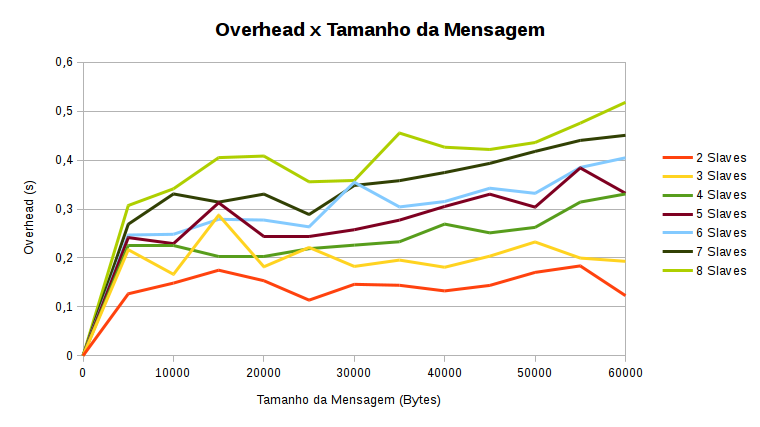
\includegraphics[scale=0.65]{figuras/overhead_distribuido.png}
\caption{Gráfico do Overhead x Tamanho da Mensagem}
\label{fig:dist:overheadXtamanho_msg}
\end{figure}

% Conclusão
% ---
\chapter{Conclusão}

Ao final desse trabalho é possível notar que um sistema distribuído é uma ferramenta muito poderosa pois permite aproveitar recursos de diferentes equipamentos para se executar uma tarefa em comum, de forma que com a distribuição do serviço entre as máquinas é consegue-se uma melhoria significativa no tempo de resposta. 

Através das análises realizadas foi possível verificar graficamente as vantagens de se realizar tarefas de forma paralela e/ou distribuída. Com essas análises também foi possível verificar alguns pontos interessantes, como o \textit{speed up} linear obtido na análise de desempenho distribuída, que é algo impossível de se obter e que pode ter sido causado pelos problemas citados, mas principalmente pelo fato de que a Lei de Amdahl considera o caso serial como sendo executado por um único processador, o que não ocorreu nesses casos visto que as máquinas possuíam mais de um \textit{core} de processamento.

Outro ponto importante e que foi possível notar durante a implementação desse trabalho é a complexidade de funcionamento que existe na máquina responsável por realizar todo o gerenciamento, nesse caso representada pelo mestre. Ele tem que lidar: com o controle de máquinas ativas, com a distribuição das tarefas, com o controle do status das tarefas, com o controle de concorrência, redistribuição de tarefas, entre outros. Além de todas essas tarefas ele ainda tem que cuidar do acesso
concorrente à variáveis de controle, que é um grande problema ao se trabalhar com muitas \textit{threads}, assim, percebe-se a necessidade que sempre vai existir para que algum pedaço do programa não seja paralelizável.


% ----------------------------------------------------------
% ELEMENTOS PÓS-TEXTUAIS
% ----------------------------------------------------------
\postextual


% ----------------------------------------------------------
% Referências bibliográficas
% ----------------------------------------------------------
%\bibliography{referencias} %% REFERENCIA AO ARQUIVO .bib

\end{document}
\grid
